\styledchapter[Inleiding]{inleiding}

NGTI is een software ontwikkel bedrijf dat gevestigd is in Rotterdam. Met het starten van nieuwe projecten begint NGTI met de probleem stelling, mockups en wireframes en prototyping. Vervolgens wordt een applicatie voor mobiel en/of webgebruik ontwikkelt en wordt support geleverd voor bijvoorbeeld updates of het oplossen van bugs \cite{ngti-services}. Naast het maken van een applicatie op maat biedt NGTI ook andere diensten, zoals een app framework of white label apps \cite{ngti-solutions}.

Kijkend naar hoe het bedrijf opereert is het een vrij 'platte' structuur. Formeel bestaat er wel een hiërarchie (\autoref{fig:ngti-organogram}), maar deze is in de praktijk niet zo gauw terug te vinden. 

\begin{figure}[hbt!]
  \centering
  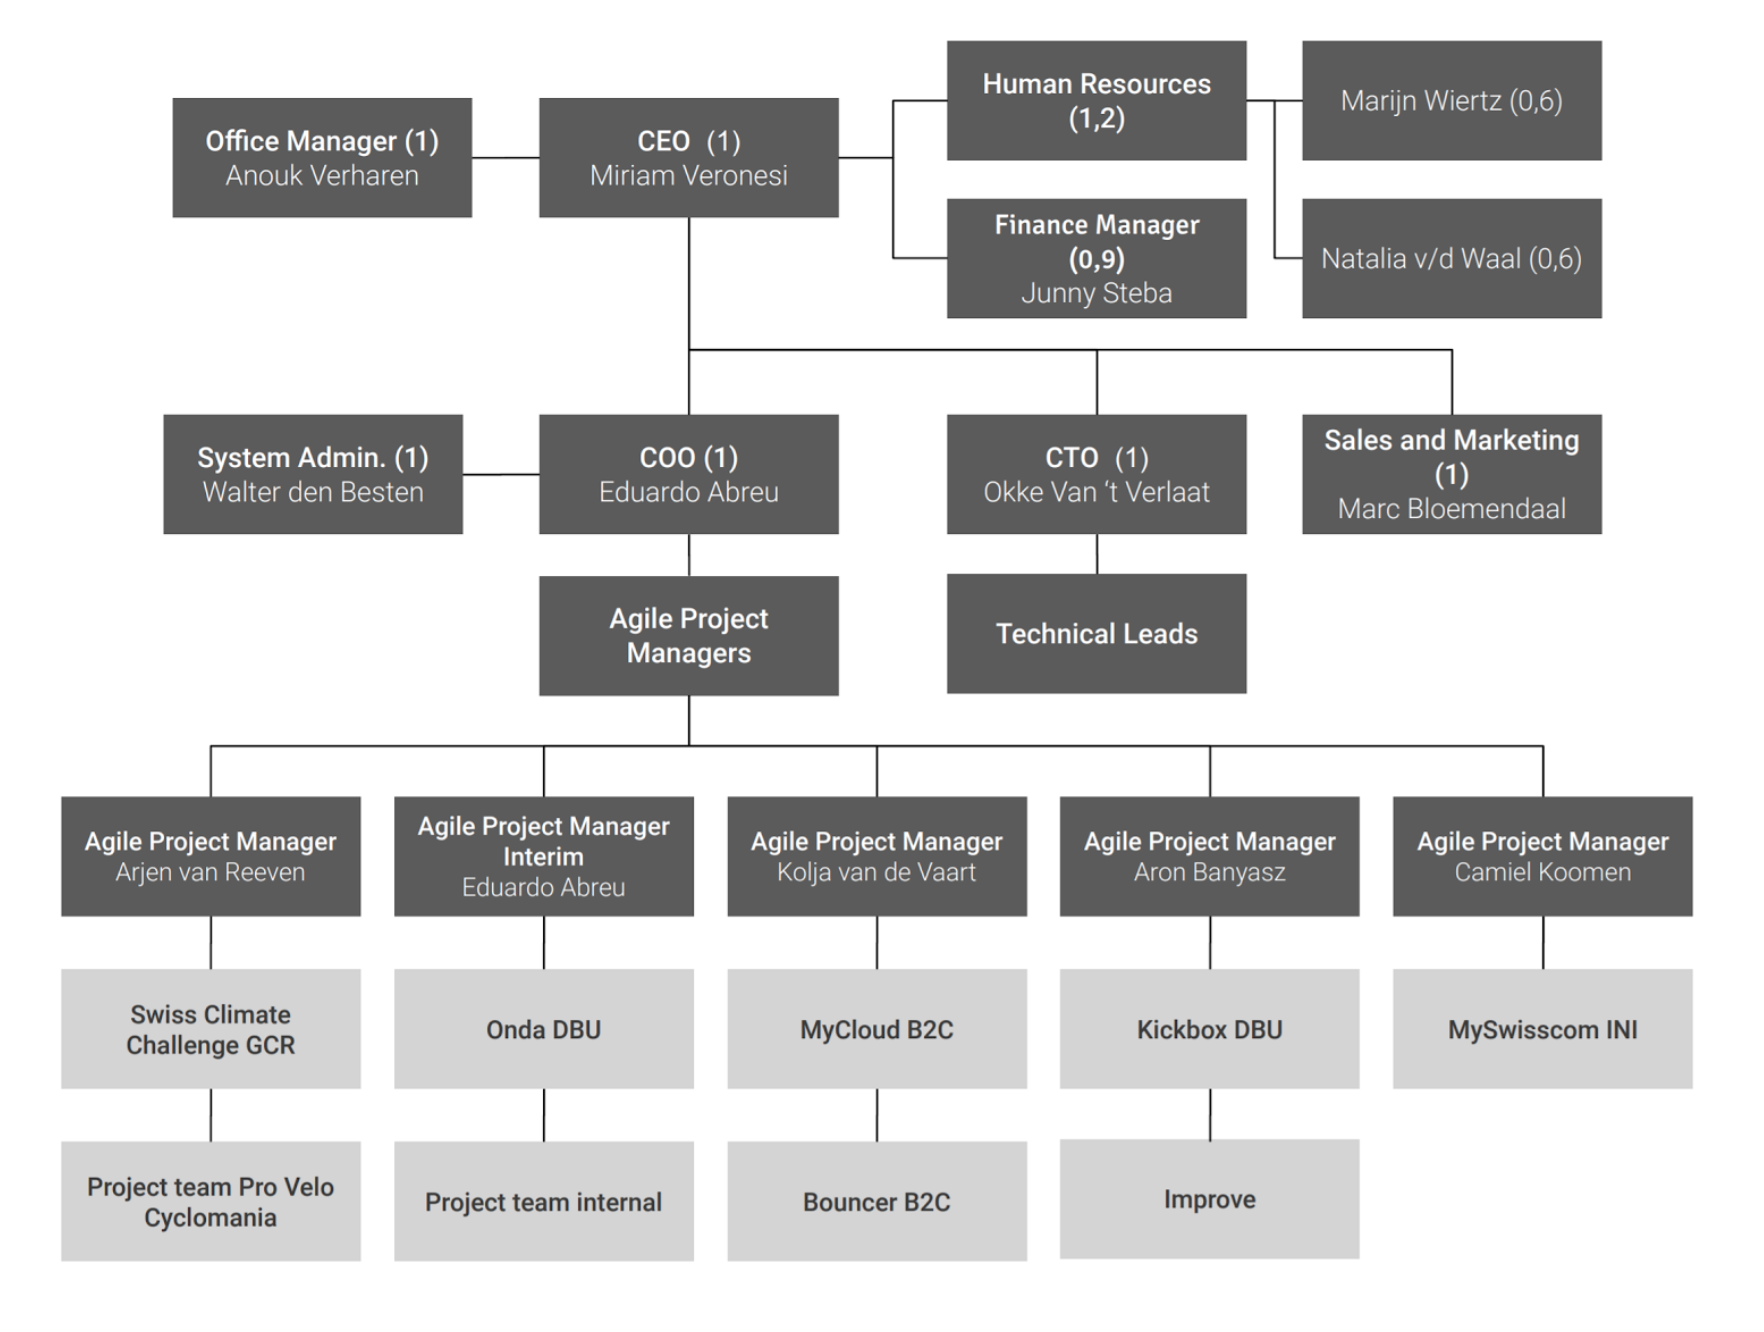
\includegraphics[width=14cm]{./chapter-1/organogram.png}
  \caption{Organogram van NGTI op 29-03-2021 \cite{ngti-organogram}.}
  \label{fig:ngti-organogram}
\end{figure}

Swisscom heeft verschillende dochterbedrijven \cite{swisscom-other-division} waarvan NGTI er een van is. Sinds maart 2021 is het bekend gemaakt dat Swisscom van plan is om een afdeling, Swisscom DevOps Center, te fuseren met NGTI. Omdat de fusie onzekerheid met zich meebrengt voor de structuur en manier hoe NGTI werkt, zal de situatie vóór de fusie aangehouden worden gedurende het afstuderen.

\section{Projecten}\label{sec:projecten}
NGTI heeft een vrij breed portfolio met apps voor verschillende doeleinden. Een van deze apps is de Climate Challenge App \cite{ngti-swisscom-climate-challenge}. Me deze app kunnen gebruikers hun C02-voetafdruk en impact in kaart brengen. Er wordt bijgehouden hoeveel kilometer de gebruiker reist en met welke vervoersmiddel. De app is onderdeel van twee bestaande nieuws apps, Blick en Bluewin \cite{swisscom-climate-challenge-integration}. Het doel is om de gebruiker aan te sporen om groener te reizen. Een screenshot van de app is te zien in \autoref{fig:swiss-climate-challenge-app}

Een andere oplossing is de My Swisscom App \cite{ngti-my-swisscom-app}. Dit is een native app voor Android en iOS waarbij Swisscom-klanten hun contract kunnen bestellen, wijzigen of beëindigen. In de app kunnen klanten ook de dataverbruik zien en instellingen voor abonnementen wijzigen. Een screenshot van de app is te zien in \autoref{fig:my-swisscom-app}.

\begin{figure}[hbt!]
  \centering
  \begin{minipage}{0.45\textwidth}
      \centering
      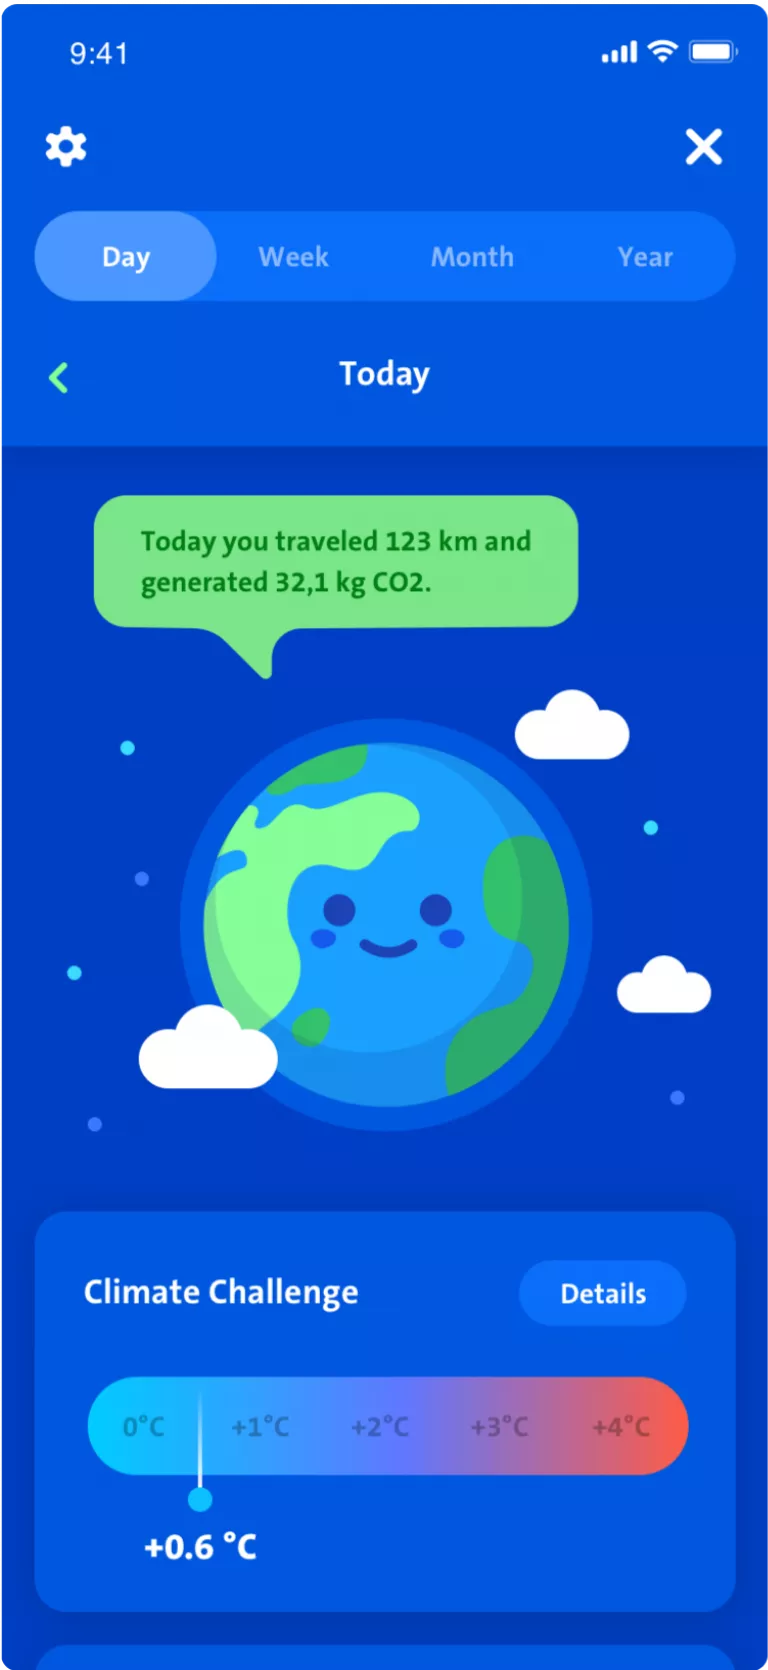
\includegraphics[width=0.65\textwidth]{./chapter-1/swiss-climate-challenge-app.png}
      \caption{Screenshot van de Swiss Climate Challenge app \cite{ngti-swisscom-climate-challenge}.}
      \label{fig:swiss-climate-challenge-app}
  \end{minipage}\hfill
  \begin{minipage}{0.45\textwidth}
      \centering
      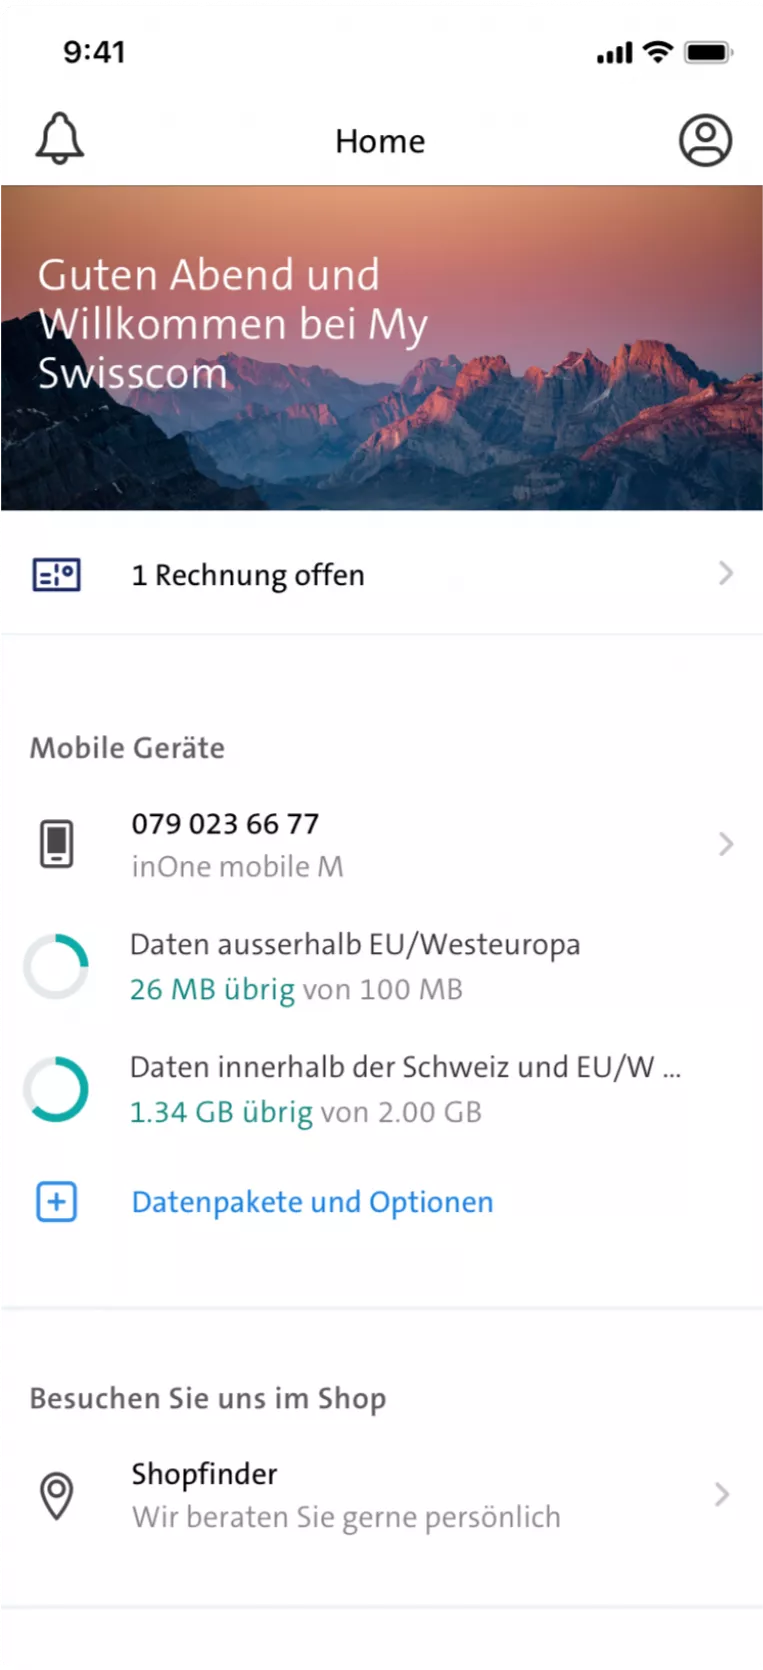
\includegraphics[width=0.65\textwidth]{./chapter-1/my-swisscom-app.png}
      \caption{Screenshot van de My Swisscom App \cite{ngti-my-swisscom-app}}
      \label{fig:my-swisscom-app}
  \end{minipage}
\end{figure}


\section{Tools die worden gebruikt}\label{sec:tools-die-gebruikt-worden}
Om productief te zijn gebruikt NGTI een aantal tools en programma's om producten te maken en te communiceren met zowel collega's als klanten. De meest gebruikte en belangrijkste zijn Slack, Google Workspace en Zoom.

\subsection{Slack}\label{subsec:slack}
Interne communicatie gaat via Slack. Het programma faciliteren collega's om elkaar met een lage instap te benaderen en berichten die voor het hele bedrijf relevant zijn te versturen. Ook zijn er 'channels' beschikbaar over specifieke onderwerpen, zoals: \textit{\#dev}, \textit{\#ios} en \textit{\#test-automation}.

\subsection{Google Workspace}\label{subsec:google-workspace}
Met Google Workspace kunnen bestanden en documenten gemaakt, opgeslagen en gedeeld worden. Omdat dit via een browser kan, hoeven werknemers geen software te installeren. NGTI gebruikt het ook om collaboratief en parallel te werken aan hetzelfde document.

\subsection{Zoom}\label{subsec:zoom}
Voorheen werd Zoom alleen gebruikt om te videobellen met collega's en geïnterviewden. In de tijd van het pandemie is Zoom echter een belangrijke speler geworden om effectief samen te werken. Meetings zoals introducties van nieuwe collega's of demo's van producten worden online gehouden.

\section{Aanleiding opdracht}\label{sec:aanleiding-opdracht}
NGTI heeft voorzien dat ze haar applicaties 'slimmer' moet maken door machine learning (ML) in te zetten. Niet alleen zorgt dit voor een betere gebruikerservaring, maar geeft NGTI ook een voorsprong op haar concurrenten.

De opdracht bestaat uit drie onderdelen:
\begin{enumerate}
  \item Onderzoek naar hoe het opzetten van een pipeline en het maken van de acties in elke stap geautomatiseerd kunnen worden
  \item Onderzoek naar hoe het trainen van een model versimpeld kan worden voor de developer
  \item Onderzoek naar het maken van een platform-agnostische oplossing
\end{enumerate}

Hierbij zal een proof-of-concept (PoC) gemaakt worden om aan te tonen of het haalbaar is. Een diepere duik in het probleem en het definiëren van de onderdelen is te vinden in \autoref{chap:probleemanalyse}.

\section{Leeswijzer}\label{sec:leeswijzer}
TODO: Schrijf leeswijzer voor elk hoofdstuk